%
% Einführung in die Mustererkennung - WS2013
% Abgabeprotokoll Exercise 1
%
%

%{{{ misc
\documentclass[subfigure,epsfig,fleqn,float,ausarbeitung]{scrartcl}

\usepackage{graphicx}
\usepackage{epstopdf}
\usepackage{caption}
\usepackage{subcaption}
\usepackage{amsmath}
\usepackage{listings}

\usepackage{pgfplots}

%Zitieren:
\usepackage[english]{babel}
%\usepackage[german]{babel}
\usepackage{babelbib} % für das Erstellen des Bibtex-Literaturverzeichnisses
\usepackage{cite}
%\selectbiblanguage{english}
%\selectbiblanguage{german}

%Peseudocode
\usepackage{algpseudocode}
\usepackage{algorithm}

%Fancy shit
\usepackage{url}

\usepackage[]{mcode}

\usepackage[pdftitle={Einfuehrung in die Mustererkennung, Exercise 3},
 						pdfauthor={Matthias Gusenbauer},
						pdfauthor={Matthias Vigele},
						pdfauthor={David Pfahler},
            pdfsubject={Mustererkennung},
            pdfborder={0 0 0}]{hyperref}


\usetikzlibrary{plotmarks}
\pgfplotsset{compat=newest} 
\pgfplotsset{plot coordinates/math parser=false}

%%%%%%%%%%%%%%%%%%%%%%%%%%%%%%%%
% Titlepage

\pagestyle{empty}


%set dimensions of columns, gap between columns, and paragraph indent

\setlength{\textheight}{24.7 cm}
\setlength{\columnsep}{1 cm}
\setlength{\textwidth}{16 cm}
%\setlength{\footheight}{0.0 cm}
\setlength{\topmargin}{0.0 cm}
\setlength{\headheight}{0.0 cm}
\setlength{\headsep}{-0.3 cm}
\setlength{\oddsidemargin}{0.0 cm}
\setlength{\parindent}{0 cm}
\setlength{\parskip}{0.5em}
\setlength{\mathindent}{0mm}

% set page counter if document is part of proceedings
\setcounter{page}{1}
\renewcommand{\floatpagefraction}{0.9}
\renewcommand{\textfraction}{0.1}

%\renewcommand{\captionlabelfont}{\fontfamily{phv}\fontseries{bx}\fontsize{10}{10pt}\selectfont}
%\renewcommand{\captionfont}{\fontfamily{phv}\fontsize{10}{12pt}\selectfont}
%\setlength{\captionmargin}{0.5 cm}

\makeatletter
\makeatother
\def\RR{\hbox{I\kern-.2em\hbox{R}}}


\begin{document}

%don't want date printed
\date{\today}

%make title bold and 14 pt font (Latex default is non-bold, 16pt) 
\title{~\\
  ~\\
  \fontsize{14}{14pt} \bf Abgabedokument Exercise 3
	 ~\\
  \fontsize{12}{12pt} \bf Einfuehrung in die Mustererkennung 186.840 WS 2013}

%for single author 
\author{~\\
  ~\\
  \fontsize{12}{12pt}
  {\bf David Pfahler, Matthias Gusenbauer, Matthias Vigele}\\
  1126287, 1125577, 1126171
  ~\\ ~\\ ~\\
  \normalsize
}

\maketitle
%I don't know why I have to reset thispagestyle, but otherwise get page numbers 
\normalfont
\thispagestyle{empty}

%%%%%%%%%%%%%%%%%%%%%%%%%%%%%%%%%%%%%%%%%%%%%%%%%%%%%%%%%%%%%%%%%%%%%%%%%%%%%%%%
% CONTENT

\stepcounter{part}
\part{The second Report}
\label{cha:secondReport}

\section{Practical Application}

\subsection{Feature Selection}

\subsection{Training- and Test-Set}

\subsection{Classification}

\subsubsection{Perceptron}

\subsubsection{Mahalanobis Distance Classifier}

\subsubsection{k-NN Classifier}

\subsection{Results}

\subsection{Discussion of the Results}


\section{Neural Network}

The following section describes the our experiences results from the neural network toolbox provided by MATLAB. This interactive toolbox can be started using the command "nnstart" to run the GUI-application as seen below.
~\\ ~\\
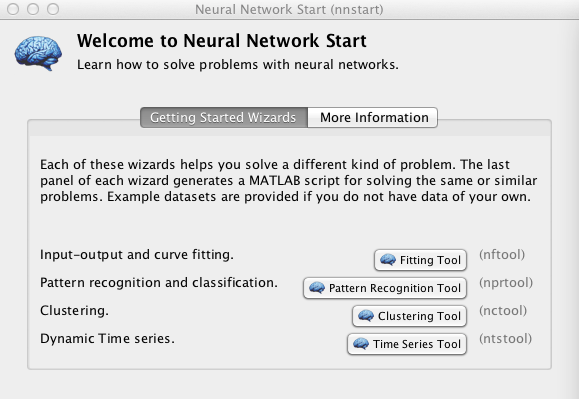
\includegraphics[scale=0.78]{img/nn/toolbox_start.png}

\subsection{Toolbox}

MATLAB offers a very intuitive way to use the neural network toolbox. You can either chose to use a graphical user interface where it is very easy to play around with different parameters. Mathworks even provided various predefined datasets ranging from medical data to wine and even the well known iris flower dataset is provided. 
~\\ ~\\
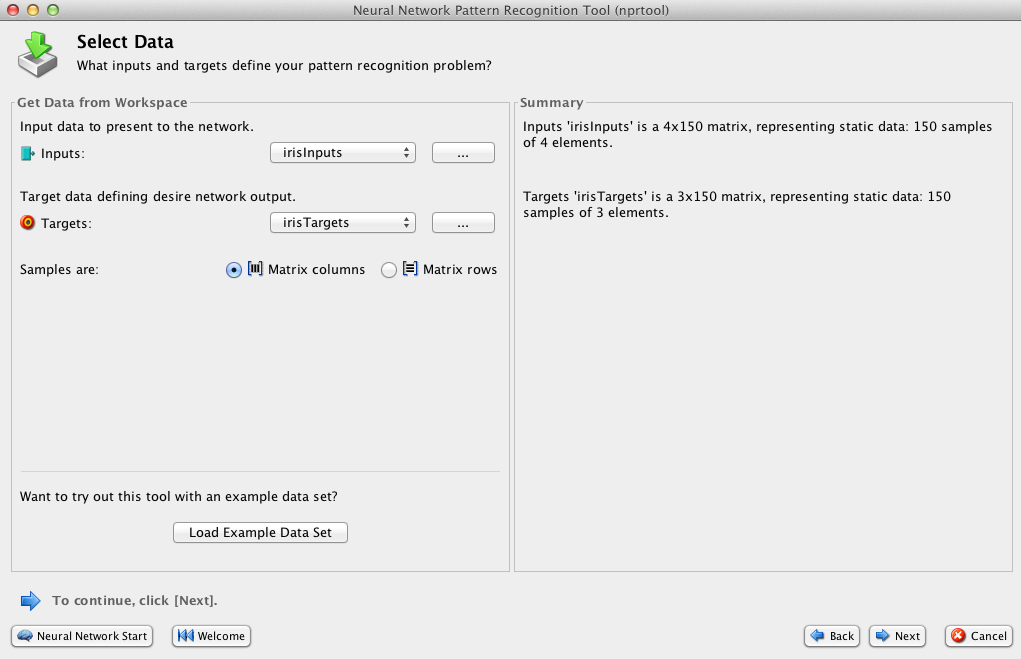
\includegraphics[scale=0.45]{img/nn/toolbox_pedef_data.png}
~\\ ~\\
The big advantage of the toolbox is not only the fact that you can solve the problem with the given UI you can change parameters, train, retrain, validate the network, create plots of the results and most important of all you there are several tools provided to dynamically create a script which does exactly what the GUI does. The benefit here is that you can seize complete control over your network. You then have the chance to change every single parameter of your network and even influence the network topology. The basic script we used for our network is taken from the the Mathworks website but was altered for our purpose. The script we use splits the training- and testset and uses another algorithm than the standard one. 

\lstset{language=Matlab, breaklines=true}

\begin{lstlisting}

function [ result ] = classifyWithNN( testData, testTarget, trainData, trainTarget )
%classifyWithNN Summary
%   For a in-depth Explanation please follow the link to the MATHWORKS 
%   documentation at: http://www.mathworks.de/de/help/nnet/gs/classify-patterns-with-a-neural-network.html

	%size of hidden layer
	hidden = 100;
      
	%create net(for pattern recognition) object
	nnet = patternnet(hidden);
      
	%set trainings algorithm
	nnet.trainFcn = 'trainrp'; %resilient backpropagation
      
	%%set up the ammount of training-, validation- and testdata
	%nnet.divideParam.trainRatio = 70/100; %70percent of the data is used for training
	%nnet.divideParam.valRatio = 15/100; %15percent for validation
	%nnet.divideParam.testRatio = 15/100; %15percent for testing
      
	%prepare data
	trainData = trainData';
	testData = testData';
      
	%train the network
	[nnet, tr] = train(nnet, trainData, trainTarget);
      
	%test the network error rate and performance
	result = nnet(testData);
	result =  (1 - (sum(vec2ind(testTarget) ~= vec2ind(result))/ numel(vec2ind(testTarget)))) * 100;

\end{lstlisting}
~\\ ~\\
As can be seen our neural network, which will be called NN from here on, has one hidden layer which consists of 100 cells. The algorithm for training is a resilient backpropagation. Another note worth mentioning is that the input data had to be transposed because the MATLAB toolbox for NN’s assumes that each column in the dataset represents one data sample and that each row equals a feature.

Another very interesting thing to mention is the fact that the Toolbox does not accept numerical values for the target values. Which means that the following vector does not produce the correct output:
~\\ ~\\
targets = $\begin{bmatrix}
1 & 1 & 2 & 2 & 3 & 3
\end{bmatrix}$
~\\ ~\\
One would assume that the first two samples are in class 1, the following two in class 2 and the last two in class 3. MATLAB however assumes another data format as standardized target vector input. In MATLAB the corresponding object would be a matrix consisting of 6 columns, one for each sample, and 3 row - one for each class. The specific matrix would look like:

~\\ ~\\
targets = 	$\begin{bmatrix}
1 & 1 & 0 & 0 & 0 & 0 \\
0 & 0 & 1 & 1 & 0 & 0\\
0 & 0 & 0 & 0 & 1 & 1
\end{bmatrix}$
~\\ ~\\

This preparation is done outside the function before the function call. The last noteworthy fact is the calculation of the result value. It seems that the NN outputs probabilities for classes and therefore we used a simple way of calculating the correct classification rate. For that we calculated the error percentage subtracted it from 1 and multiplied that value by 100 to get the percentage of correctly classified samples.

\subsection{Results}

To get valid results we randomized the training and test data and performed the classification multiple times to get a more realistic image of the performance of the NN applied on the given problem. The classification rate is very stable at 67 percent and above. The top measured performance is 75 percent. This result was achieved after the NN was trained for about 30 epochs each time. 
The classification runs two times. The first time with all features and the second time with the best features according to the principle component analysis which was done beforehand. The results of the first test run with the full set of features were 75,3\% correct classification for the dry- versus wet strokes and 67,6\% for the classification problem with all six classes. 
For the second test run with only the significant features the results were 73,5\% for the two class problem and 67,1\% for the problem with six classes.

\subsection{Discussion of the Results}

A very interesting discovery is that for the NN it seems that it does not matter whether it gets trained on “good” features or on the full set. The results are very similar and the full set leads even leads to an slightly better result. A very important discovery was that the cell count of the hidden layer of the NN is very important for the quality of results. For our results we used 100 cells in the hidden layer. When we tried to improve our results we tried to increase the hidden layer size. 
The first try was 500 cells and we immediately got worse results. The result for the good features and 6 classes even dropped to a percentage of 9,9 and the number of epochs during training ranged from 6 to 27.
For the second try we set the cell count to 10 and the worst result was 64,1\% for the PCA features and the 6 classes. It seems that the decrease of the hidden layer size up to a point does not harm the NN as much as the increase which may be the case because too many cells in the hidden layer lead to over fitting of the NN on the training set. Another disadvantage of too many cells is the computing time. With a bigger hidden layer the amount to compute for training, validation and testing increases as well and then the run time performance drops.

\end{document}

% vim:foldmethod=marker
